% Provenance (never printed): see sources/outline_sources.md (Year 2: the vanished ocean;
% ophiolites; nappes; high-pressure rocks; foreland basins; reconstructing the history from
% maps, sections and geophysics). Units, ages and architecture after Schmid et al. (2004);
% Monte Cervino sheet notes (ISPRA 2016); Penrose definition as quoted by Coleman (1984);
% Zermatt-Saas ages Rubatto et al. (1998), Halama et al. (2020); Chenaillet Corno et al.
% (2023); Moho picks Michailos et al. (2023, Zenodo, CC BY 4.0); gravity Zahorec et al.
% (2021); Jura Lanza et al. (2022), Schori et al. (2015); shortening Rosenberg et al.
% (2021); Glarus thrust Herwegh et al. (2008); Molasse Krenmayr (1999), Garefalakis and
% Schlunegger (2018), Sinclair (1997); present uplift Champagnac et al. (2009). Figure data
% in figdata/bachelor-2/alps.py; exercise and problem values in the Book 4 scratch
% calculator calc/ch13.py.
\chapter{Anatomia de um cinturão de montanhas: os Alpes}\label{ch:b2:alpine-orogen}

O cume do Matterhorn é feito de gnaisse e gabro que pertenceram um dia à margem
da Apúlia, o continente que ficava do lado da África de um oceano desaparecido. As encostas abaixo
dele são o fundo desse oceano, serpentinito, gabro e basalto em almofada transformados em eclogito, e,
por baixo, no vizinho Monte Rosa, está a borda da Europa. Escalando a
pilha, passa-se de um continente, através de um oceano, ao outro. Este capítulo lê os Alpes como uma pilha assim: de onde vieram suas peças, como elas foram
empilhadas, quanto terreno o empilhamento consumiu e o que a geofísica vê por baixo.
% ledger: ispra16:cervino, schmid04:apulia, schmid04:alpine-tethys

\begin{recall}
\textbf{Do volume do ensino médio}: a colisão continental, a sutura, o encurtamento de uma
camada (a fração do seu comprimento perdida), as falhas inversas e os cavalgamentos. \textbf{Do volume do primeiro
ano}: mapas e seções geológicas; falhas normais, inversas e de empurrão, dobras e
vergência; as margens passivas; a crosta oceânica, a lava em almofada e o complexo de \omterm{def:b2:magma-emplacement:bodies}{diques} em lençol;
as margens ativas e o prisma de acreção; a isostasia, a raiz de Airy e a anomalia de Bouguer;
a \omterm{def:b2:alpine-orogen:foreland}{bacia de antepaís}, citada entre as bacias sedimentares. \textbf{Do
\cref{ch:b2:metamorphic-facies}}: as fácies xisto azul e eclogito. \textbf{Do
\cref{ch:b2:pt-paths}}: \omterm{def:b2:pt-paths:ptt}{trajetórias P--T--t}, \omterm{def:b2:pt-paths:exhumation}{taxas de exumação} e \omterm{def:b2:pt-paths:uhp}{metamorfismo de
ultra-alta pressão}.
\end{recall}

\begin{definition}[Orógeno]\label{def:b2:alpine-orogen:orogen}
Um \emph{orógeno}\index{orógeno} é um cinturão da litosfera encurtado e espessado pela
convergência de duas placas, junto com as rochas deformadas e metamorfizadas nele; a
cadeia de montanhas é sua expressão em superfície, a crosta espessada por baixo é sua raiz.
\end{definition}

\section{Um oceano desaparecido}\label{sec:b2:alpine-orogen:tethys}

Os Alpes registram o fechamento de oceanos enquanto as placas africana e europeia convergiam.
O principal é o \emph{Tétis Alpino}, formado por dois ramos. Seu ramo sul, o
oceano Piemonte--Ligúria, começou a se abrir no Jurássico Médio, quando o Atlântico Central
se abriu: o Tétis Alpino pertence cinematicamente à abertura do Atlântico, ao contrário dos
oceanos tetianos mais a leste. Radiolaritos, vasas silicosas do mar profundo transformadas em rocha,
e calcários de aptychus seguiram o início da expansão, e ainda hoje identificam seus
restos. Um ramo norte estreito, o oceano do Valais, provavelmente se abriu no início do
Cretáceo. Entre os dois havia uma lasca de continente, a faixa do Briançonnais, que se adelgaça
para leste e está ausente dos Alpes orientais.
% ledger: schmid04:alpine-tethys

Ao norte, o oceano era limitado pela margem passiva da Europa, assunto do capítulo de rifts e
margens do volume do primeiro ano. Ao sul ficava a \emph{Apúlia}: todo o terreno continental
ao sul do Tétis Alpino e ao norte do Neotétis, mais jovem, incluindo o antepaís
que hoje fica ao sul dos Alpes. O cume do Matterhorn é um pedaço dela.
% ledger: schmid04:apulia
O mapa abaixo situa o cinturão e os lugares deste capítulo.

\begin{omfigure}
\centering
% ledger: data:b4-etopo-alps, schmid04:windows, schmid04:foreland, ispra16:cervino
\begin{tikzpicture}
\begin{axis}[width=0.96\linewidth, height=0.74\linewidth, xmin=5, xmax=14, ymin=43.5,
  ymax=48.5, xlabel={longitude (\unit{\degree} L)}, ylabel={latitude (\unit{\degree} N)},
  tick label style={font=\scriptsize}, label style={font=\small}, clip=true,
  xtick={5,6,...,14}, ytick={44,45,...,48}]
\addplot[omThm!35, line width=0.3pt] table[x=lon, y=lat] {figdata/out/bachelor-2-alps-c1000.dat};
\addplot[omThm!90!black, line width=0.45pt] table[x=lon, y=lat] {figdata/out/bachelor-2-alps-c2000.dat};
\addplot[blue!60!black, line width=0.5pt] table[x=lon, y=lat] {figdata/out/bachelor-2-alps-c0.dat};
\draw[red!70!black, line width=1pt] (axis cs:8,45.3) -- (axis cs:8,48.0);
\node[font=\scriptsize\bfseries, red!70!black, anchor=north west] at (axis cs:8.02,45.32) {A};
\node[font=\scriptsize\bfseries, red!70!black, anchor=south west] at (axis cs:8.02,47.98) {B};
\fill (axis cs:6.865,45.833) circle (1.3pt) node[font=\scriptsize, fill=white, fill opacity=0.85, text opacity=1, inner sep=1pt, anchor=north east] {Mont Blanc};
\fill (axis cs:7.659,45.976) circle (1.3pt) node[font=\scriptsize, fill=white, fill opacity=0.85, text opacity=1, inner sep=1pt, anchor=south east] {Matterhorn};
\node[font=\scriptsize\itshape, rotate=40] at (axis cs:6.35,46.85) {Jura};
\node[font=\scriptsize\itshape] at (axis cs:9.35,47.65) {bacia da Molassa};
\node[font=\scriptsize\itshape] at (axis cs:10.0,45.05) {planície do Pó};
\node[font=\scriptsize\itshape, align=center, fill=white, fill opacity=0.8, text opacity=1, inner sep=1pt] at (axis cs:10.3,46.95) {janela da\\Engadina};
\node[font=\scriptsize\itshape, align=center, fill=white, fill opacity=0.8, text opacity=1, inner sep=1pt] at (axis cs:12.6,47.25) {janela dos\\Tauern};
\node[font=\scriptsize\itshape] at (axis cs:8.6,43.85) {mar da Ligúria};
\end{axis}
\end{tikzpicture}
\par\smallskip{\small Os Alpes no modelo de relevo ETOPO1, com os nós a \qty{0.05}{\degree}
uns dos outros: curvas de nível de \qty{1000}{m} (claro) e \qty{2000}{m} (escuro) e a linha de costa. O
nó mais alto desta grade tem \qty{3914}{m}, perto do Mont Blanc; os cumes são mais altos,
porque um nó da grade amostra uma célula, não um pico. A linha A--B ao longo de \qty{8}{\degree} L é
o perfil traçado na última seção do capítulo. Nomes dos acidentes colocados à mão em suas
posições aproximadas.}
\end{omfigure}

Como se pode conhecer um oceano que desapareceu? Por pedaços do seu fundo que escaparam à
subducção e foram presos no cinturão de montanhas.

\begin{definition}[Ofiolito; sequência ofiolítica de Penrose]\label{def:b2:alpine-orogen:ophiolite}
Um \emph{ofiolito}\index{ofiolito} é uma associação característica de rochas máficas a
ultramáficas, um pedaço de litosfera oceânica hoje encontrado em terra. A \emph{sequência ofiolítica
de Penrose}\index{sequência ofiolítica de Penrose} é a associação completa definida por uma
conferência de geólogos em 1972; da base para o topo:
\begin{enumerate}
\item um complexo ultramáfico de \omterm{def:b2:mantle-melting:peridotites}{harzburgito}, \omterm{def:b2:mantle-melting:peridotites}{lherzolito} e \omterm{def:b2:mantle-melting:peridotites}{dunito}, geralmente com uma
trama de deformação adquirida no estado sólido;
\item um complexo gabroico, em geral com texturas de \omterm{def:b2:magmatic-differentiation:cumulate}{cumulato};
\item um complexo máfico de \omterm{def:b2:magma-emplacement:bodies}{diques} em lençol;
\item um complexo vulcânico máfico, comumente em almofadas.
\end{enumerate}
\end{definition}
% ledger: coleman84:penrose

A definição de Penrose foi um consenso, criticado desde o início e ainda geralmente
aceito. Sua sequência é o acamamento da crosta oceânica e do manto superior visto no volume do primeiro
ano: lavas em almofada sobre \omterm{def:b2:magma-emplacement:bodies}{diques} em lençol sobre gabro sobre o manto. Os \omterm{def:b2:alpine-orogen:ophiolite}{ofiolitos}, porém, não são
um fundo oceânico médio. A maior parte da crosta abissal, a crosta dos oceanos largos, é consumida pela
subducção; Coleman argumentou que os \omterm{def:b2:alpine-orogen:ophiolite}{ofiolitos} dos cinturões alpino e cordilheirano se formaram
principalmente nos centros de expansão de pequenas bacias oceânicas ou entre arcos insulares, e que os
tetianos se formaram onde a crosta continental se afinou ao longo de margens passivas até que um pequeno
oceano se abrisse.
% ledger: coleman84:penrose, coleman84:settings

Os \omterm{def:b2:alpine-orogen:ophiolite}{ofiolitos} alpinos se encaixam nesse quadro. As unidades derivadas do oceano Piemonte--Ligúria
são relíquias de litosfera oceânica e de manto trazido de baixo do continente
afinado, o manto subcontinental, e exposto no fundo do mar. No
Chenaillet, nos Alpes Ocidentais, o mais bem preservado deles mostra manto
exposto, gabros e uma famosa sequência de basaltos em almofada, sem cobertura sedimentar.
A fotografia abaixo os mostra.
% ledger: schmid04:units, corno23:chenaillet

\begin{omfigure}
\centering
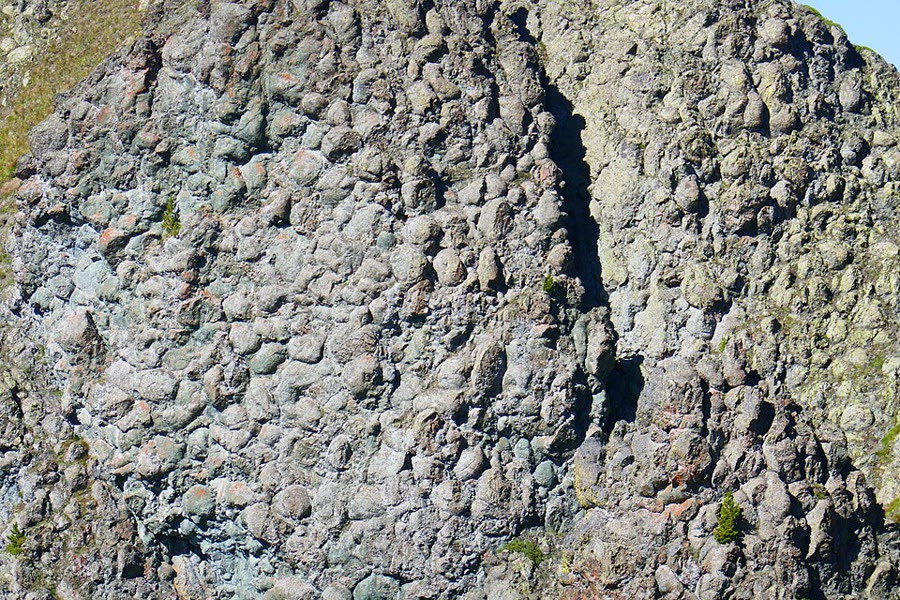
\includegraphics[width=0.66\linewidth]{images/book4/b2-13-pillow-lava.jpg}
\par\smallskip{\small Lavas em almofada do \omterm{def:b2:alpine-orogen:ophiolite}{ofiolito} do Chenaillet, Alpes Ocidentais: cada
almofada arredondada é um lobo de basalto que irrompeu e se resfriou no fundo do oceano
Piemonte--Ligúria. Fotografia de Lionel Duchoiselle, CC BY-SA 3.0.}
\end{omfigure}

O fundo oceânico pode ser datado onde seus gabros se cristalizaram. Zircões de dois metagabros do
\omterm{def:b2:alpine-orogen:ophiolite}{ofiolito} de Zermatt--Saas, abaixo do Matterhorn, dão $164.0 \pm \qty{2.7}{Ma}$ e $163.5
\pm \qty{1.8}{Ma}$, e os sedimentos ricos em manganês depositados sobre os basaltos têm no máximo $161
\pm \qty{11}{Ma}$: o fundo do oceano Piemonte--Ligúria estava se formando no Jurássico,
há cerca de \qty{164}{Myr}.
% ledger: rubatto98:zsf

\section{Subductar um oceano, depois um continente}\label{sec:b2:alpine-orogen:subduction}

Um oceano se fecha por subducção. Parte do seu fundo, porém, acaba por cima de um continente
em vez de por baixo dele, e alguns continentes seguem o oceano para baixo.

\begin{definition}[Obducção; subducção continental]\label{def:b2:alpine-orogen:obduction}
A \emph{obducção}\index{obducção} é o alojamento de uma placa de litosfera oceânica sobre
uma margem continental, o \omterm{def:b2:alpine-orogen:ophiolite}{ofiolito} cavalgando o continente. A \emph{subducção
continental}\index{subducção continental} é a descida de litosfera continental, puxada
pela laje oceânica ligada a ela, numa zona de subducção depois que o oceano à sua frente
foi consumido.
\end{definition}

Houve \omterm{def:b2:alpine-orogen:obduction}{obducção} nos Dinarides, a sudeste dos Alpes: \omterm{def:b2:alpine-orogen:ophiolite}{ofiolitos} do oceano jurássico de
Vardar, eles próprios do Jurássico Médio, foram cavalgados no Jurássico Superior sobre um
prisma de acreção e sobre a margem da Apúlia. Por muito tempo pensou-se que ela tinha alojado também o
\omterm{def:b2:alpine-orogen:ophiolite}{ofiolito} do Chenaillet, porque suas rochas mostram apenas um \omterm{def:b2:metamorphic-facies:metamorphism}{metamorfismo} alpino de grau muito
baixo. Um estudo recente encontrou relíquias de lawsonita e onfacita em seu gabro e em seu
albitito, que situam seu pico alpino a 10 a \qty{11}{kbar} e 340 a
\qty{360}{\celsius}: o peso de uma \omterm{def:b2:alpine-orogen:nappes}{pilha de nappes} de uns 35 a \qty{40}{km} de espessura. Os autores
concluem que o Chenaillet foi subductado, não obductado, um lembrete de que a leitura de
um \omterm{def:b2:alpine-orogen:ophiolite}{ofiolito} depende tanto de sua história metamórfica quanto de suas rochas.
% ledger: schmid04:obduction, corno23:chenaillet

\subsection*{O oceano desce}

No Cretáceo, a margem sul, apuliana, do oceano Piemonte--Ligúria tornou-se uma
margem ativa: sua fossa se encheu de folhelhos e arenitos, hoje os xistos calcários
chamados Bündnerschiefer ou schistes lustrés. Os Alpes orientais registram também uma colisão
anterior, o fechamento de um golfo de outro oceano, o Meliata, contra a Apúlia, com um
pico de alta pressão por volta de \qty{100}{Ma}: os Alpes são o produto de duas orogenias, uma
cretácea e uma terciária.
% ledger: schmid04:two-orogenies

O \omterm{def:b2:alpine-orogen:ophiolite}{ofiolito} de Zermatt--Saas desceu até a fácies eclogito do
\cref{ch:b2:metamorphic-facies}: seus eclogitos atingiram 550 a \qty{600}{\celsius} e 2.5 a
\qty{3.0}{GPa}, e o pico de pressão foi atingido entre 48 e \qty{44}{Ma}. Uma lasca dele,
em Lago di Cignana, contém coesita e diamantes microscópicos em rochas que começaram como basaltos
e sedimentos do fundo oceânico; ela atingiu cerca de \qty{615}{\celsius} e \qty{2.8}{GPa}, e seus
zircões datam esse ponto mais profundo em $44.1 \pm \qty{0.7}{Ma}$. Um fundo oceânico nascido
há \qty{164}{Myr} foi subductado, com a idade de 120 milhões de anos, a profundidades de
\qty{90}{km} ou mais, e depois voltou.
% ledger: halama20:cignana, rubatto98:zsf

\subsection*{O continente vem atrás}

Quando o oceano desapareceu, a margem da Europa foi arrastada atrás dele. Os quartzitos com
coesita do maciço de Dora Maira, vistos no \cref{ch:b2:pt-paths}, são crosta continental
do lado europeu do oceano que chegou a mais de \qty{90}{km}, há cerca de
\qty{35}{Myr}, e voltou à velocidade das placas. Datar as rochas de alta pressão
através do cinturão dá uma ordem: a própria margem apuliana (a zona Sesia) no Cretáceo
Superior, os \omterm{def:b2:alpine-orogen:ophiolite}{ofiolitos} do oceano Piemonte--Ligúria por volta de \qty{44}{Ma}, a
crosta continental europeia no Eoceno Superior. Rubatto e colaboradores a leem como três episódios de subducção que avançam no tempo de
sudeste para noroeste, em direção à Europa.
% ledger: chopin84:coesite, rh01:exhumation, rubatto98:zsf, ispra16:cervino

Seguiu-se a colisão: o oceano do Valais, a última faixa oceânica, fechou-se do Eoceno Médio ao
Superior, e a partir daí crosta continental foi empilhada sobre crosta continental.
A figura abaixo resume a sequência.
% ledger: schmid04:alpine-tethys

\begin{omfigure}
\centering
\begin{tikzpicture}[x=0.95cm, y=0.78cm, font=\scriptsize]
% (a) rifting and spreading
\begin{scope}[yshift=0cm]
\node[anchor=west, font=\scriptsize\bfseries] at (-0.2,0.75) {(a) Jurássico: o oceano se abre};
\fill[gray!25] (0,0) -- (3.2,0) -- (3.8,-0.6) -- (0,-0.6) -- cycle;
\fill[gray!25] (6.2,0) -- (10,0) -- (10,-0.6) -- (5.6,-0.6) -- cycle;
\fill[omThm!35] (3.2,0) -- (6.2,0) -- (5.6,-0.6) -- (3.8,-0.6) -- cycle;
\fill[blue!8] (0,0) rectangle (10,0.4);
\draw[thick] (4.7,0) -- (4.7,-0.6);
\node at (1.6,-0.3) {Europa};
\node at (8,-0.3) {Apúlia};
\node[align=center] at (4.7,0.2) {dorsal};
\end{scope}
% (b) oceanic subduction
\begin{scope}[yshift=-1.7cm]
\node[anchor=west, font=\scriptsize\bfseries] at (-0.2,0.75) {(b) Cretáceo a Eoceno: o oceano é subductado};
\fill[blue!8] (0,0) rectangle (7,0.4);
\fill[gray!25] (0,0) -- (3.0,0) -- (3.6,-0.6) -- (0,-0.6) -- cycle;
\fill[omThm!35] (3.0,0) -- (6.3,0) -- (6.0,-0.5) -- (5.6,-0.95) -- (3.6,-0.6) -- cycle;
\fill[gray!25] (6.3,0) -- (6.6,0.3) -- (10,0.3) -- (10,-0.6) -- (6.4,-0.6) -- cycle;
\fill[omThm!35] (5.6,-0.95) -- (6.0,-0.5) -- (7.4,-1.3) -- (7.2,-1.55) -- cycle;
\fill[orange!40] (6.0,0) -- (6.3,0) -- (6.6,0.3) -- (6.35,0.3) -- cycle;
\draw[-{Latex[length=2mm]}] (7.0,-1.0) -- (7.6,-1.38);
\node at (1.6,-0.3) {Europa};
\node at (8.4,-0.15) {Apúlia};
\node[anchor=west] at (7.5,-1.1) {eclogito};
\end{scope}
% (c) continental subduction
\begin{scope}[yshift=-3.95cm]
\node[anchor=west, font=\scriptsize\bfseries] at (-0.2,0.75) {(c) Eoceno: a margem europeia vem atrás};
\fill[gray!25] (0,0) -- (5.6,0) -- (6.2,-0.5) -- (7.4,-1.35) -- (7.1,-1.6) -- (5.6,-0.6) -- (0,-0.6) -- cycle;
\fill[omThm!35] (6.2,0.05) -- (6.6,0.3) -- (6.95,0.3) -- (6.4,-0.2) -- cycle;
\fill[gray!25] (6.6,0.3) -- (10,0.3) -- (10,-0.6) -- (6.9,-0.6) -- (6.4,-0.2) -- (6.95,0.3) -- cycle;
\draw[dashed] (6.6,-0.85) circle (0.22);
\draw (6.82,-0.9) -- (7.6,-1.2);
\node[anchor=west] at (7.6,-1.2) {crosta continental de UHP};
\node at (2.4,-0.3) {Europa};
\node at (8.4,-0.15) {Apúlia};
\end{scope}
% (d) collision
\begin{scope}[yshift=-6.65cm]
\node[anchor=west, font=\scriptsize\bfseries] at (-0.2,1.4) {(d) Oligoceno ao presente: colisão, nappes, bacias de antepaís};
\fill[yellow!35] (0.6,0) -- (3.4,0) -- (3.4,-0.3) -- cycle;
\fill[gray!25] (0,-0.3) -- (3.4,-0.3) -- (4.2,0.5) -- (5.2,0.75) -- (6.2,0.55) -- (7.0,0.2) -- (10,0.2)
  -- (10,-0.7) -- (6.6,-0.7) -- (5.4,-1.5) -- (4.0,-1.5) -- (3.2,-0.9) -- (0,-0.9) -- cycle;
\draw (3.4,-0.3) -- (4.5,-1.0);
\draw (4.2,0.5) -- (5.6,-0.4);
\draw (5.2,0.75) -- (6.1,0.1);
\fill[omThm!35] (5.05,0.6) -- (5.55,0.68) -- (5.85,0.32) -- (5.4,0.25) -- cycle;
\fill[yellow!35] (7.0,0.2) -- (9.6,0.2) -- (7.0,-0.1) -- cycle;
\node at (1.4,-0.6) {Europa};
\node at (8.6,-0.3) {Apúlia};
\node[anchor=south] at (1.9,0.02) {molassa};
\node at (4.7,-1.25) {raiz};
\node[anchor=south west] at (6.25,0.6) {pilha de nappes};
\end{scope}
\end{tikzpicture}
\par\smallskip{\small Uma história esquemática dos Alpes, fora de escala (litosfera oceânica em vermelho,
continental em cinza, prisma de acreção em laranja, \omterm{def:b2:alpine-orogen:foreland}{bacias de antepaís} em amarelo).
(a)~O oceano Piemonte--Ligúria se abre entre a Europa e a Apúlia. (b)~Seu fundo é subductado
sob a Apúlia e transformado em eclogito. (c)~A margem europeia é puxada para baixo atrás dele e
metamorfizada em ultra-alta pressão. (d)~A crosta continental é empilhada em \omterm{def:b2:alpine-orogen:nappes}{nappes} sobre uma
raiz espessada, com \omterm{def:b2:alpine-orogen:foreland}{bacias de antepaís} flexurais dos dois lados.}
\end{omfigure}
% ledger: schmid04:alpine-tethys, schmid04:two-orogenies, rubatto98:zsf, schmid04:foreland

\section{Nappes, klippen e janelas}\label{sec:b2:alpine-orogen:nappes}

As peças de oceano e de continente não foram empilhadas inteiras. Foram raspadas em finas
lâminas e levadas para longe.

\begin{definition}[Nappe; pilha de nappes]\label{def:b2:alpine-orogen:nappes}
Uma \emph{nappe}\index{nappe} é uma grande lâmina de rocha, frequentemente com alguns quilômetros de espessura e dezenas
de quilômetros de comprimento, transportada ao longo de um cavalgamento de baixo ângulo ou no flanco invertido de uma grande
dobra deitada para longe do seu lugar de origem; as rochas de uma nappe são
\emph{alóctones}\index{alóctone (unidade rochosa)}, as que ficaram no lugar,
\emph{autóctones}\index{autóctone (unidade rochosa)}. Uma \emph{pilha de
nappes}\index{pilha de nappes} é um empilhamento de nappes no qual as nappes estruturalmente mais altas
geralmente vêm de mais para dentro do \omterm{def:b2:alpine-orogen:orogen}{orógeno}.
\end{definition}

Nos Alpes, a ordem de empilhamento é a geografia do oceano desaparecido virada de cabeça para baixo,
e as unidades são nomeadas por sua origem (tabela abaixo).

\begin{omfigure}
\centering\small
\begin{tabular}{>{\raggedright\arraybackslash}p{0.24\linewidth}|>{\raggedright\arraybackslash}p{0.66\linewidth}}
unidade (do topo à base) & origem e rochas \\ \hline
\omterm{def:b2:alpine-orogen:nappes}{Nappes} austroalpinas & margem da Apúlia ao norte da Linha Periadriática: lascas de embasamento e de cobertura
destacadas de sua crosta inferior \\
\omterm{def:b2:alpine-orogen:nappes}{Nappes} Margna--Sesia (zona Sesia, Dent Blanche) & fragmentos separados por rifte da margem
apuliana mais externa quando o oceano se abriu \\
\omterm{def:b2:alpine-orogen:nappes}{Nappes} peninicas superiores & oceano Piemonte--Ligúria: \omterm{def:b2:alpine-orogen:ophiolite}{ofiolitos}, manto exumado, xistos
calcários \\
\omterm{def:b2:alpine-orogen:nappes}{Nappes} peninicas médias & o microcontinente em faixa do Briançonnais \\
\omterm{def:b2:alpine-orogen:nappes}{Nappes} peninicas inferiores & oceano do Valais: \omterm{def:b2:alpine-orogen:ophiolite}{ofiolitos} e xistos calcários \\
\omterm{def:b2:alpine-orogen:nappes}{Nappes} subpeninicas & embasamento europeu destacado de sua crosta inferior \\
\omterm{def:b2:alpine-orogen:nappes}{Nappes} helvéticas & cobertura rica em calcário da margem europeia próxima, destacada do seu
embasamento \\ \hline
Alpes Meridionais & Apúlia ao sul da Linha Periadriática: um \omterm{def:b2:alpine-orogen:ftb}{cinturão de dobras e cavalgamentos} com vergência para o sul,
sobretudo miocênico, de 10 a \qty{15}{km} de espessura
\end{tabular}
\par\smallskip{\small As principais unidades tectônicas dos Alpes, do topo estrutural
para baixo, com o domínio de onde cada uma veio (segundo Schmid e colaboradores).}
\end{omfigure}
% ledger: schmid04:units, schmid04:apulia

A placa superior, a Apúlia, fica por cima; abaixo dela vêm, em ordem, o oceano distante, o
Briançonnais, o oceano próximo e a margem europeia, sendo as unidades mais baixas as que
estavam mais perto da Europa. Grandes dobras que redobraram as \omterm{def:b2:alpine-orogen:nappes}{nappes} depois de empilhadas
às vezes perturbam a ordem, e algumas lascas, como o Briançonnais, se acunham ao longo do
cinturão.
% ledger: schmid04:units, schmid04:alpine-tethys

A erosão então corta a pilha, e duas formas aparecem num mapa.

\begin{definition}[Klippe; janela tectônica]\label{def:b2:alpine-orogen:klippe}
Uma \emph{klippe}\index{klippe} (plural klippen) é um resto isolado de uma \omterm{def:b2:alpine-orogen:nappes}{nappe}, que ficou
de pé sobre as rochas abaixo dela quando a erosão removeu o resto da lâmina; ela é
cercada por seu cavalgamento basal. Uma \emph{janela tectônica}\index{janela tectônica} é um buraco
aberto pela erosão através de uma \omterm{def:b2:alpine-orogen:nappes}{nappe}, onde aparecem as rochas abaixo do seu cavalgamento basal, cercado pela
\omterm{def:b2:alpine-orogen:nappes}{nappe}.
\end{definition}

\begin{omfigure}
\centering
\begin{tikzpicture}[x=0.68cm, y=0.68cm, font=\scriptsize]
\def\thrust{(0,0) -- (5,0) .. controls (6.5,0) and (7,1.1) .. (8,1.1)
  .. controls (9,1.1) and (9.5,0) .. (11,0) -- (16,0)}
\def\topo{(0,1.7) .. controls (3,1.9) and (5,1.8) .. (6,1.5) .. controls (7,1.0) .. (8,0.6)
  .. controls (9,1.0) .. (10.3,1.5) .. controls (11.3,1.3) .. (12.5,-0.4)
  .. controls (13.3,0.9) .. (14.5,0.95) .. controls (15.5,0.8) .. (16,-0.2)}
\begin{scope}
\clip \topo -- (16,-2.6) -- (0,-2.6) -- cycle;
\fill[gray!20] (0,-2.6) rectangle (16,2.2);
\fill[omThm!30] \thrust -- (16,2.2) -- (0,2.2) -- cycle;
\draw[gray!55, yshift=-0.9*0.68cm] \thrust;
\draw[gray!55, yshift=-1.8*0.68cm] \thrust;
\draw[line width=1.2pt] \thrust;
\end{scope}
\draw \topo;
\node at (2.5,1.0) {nappe};
\node[anchor=north west] at (0.2,-0.05) {cavalgamento basal};
\node at (3.6,-1.35) {autóctone};
\draw[-{Latex[length=1.6mm]}] (8,2.0) node[anchor=south] {janela tectônica} -- (8,0.75);
\draw[-{Latex[length=1.6mm]}] (14.5,2.0) node[anchor=south] {klippe} -- (14.5,1.05);
\end{tikzpicture}
\par\smallskip{\small Uma \omterm{def:b2:alpine-orogen:nappes}{nappe} (em cor) sobre o seu autóctone (cinza) depois da erosão, numa
seção esquemática: onde seu cavalgamento basal (linha grossa) se arqueia, a erosão cortou
a \omterm{def:b2:alpine-orogen:nappes}{nappe} e abriu uma \omterm{def:b2:alpine-orogen:klippe}{janela tectônica} para as rochas de baixo; na frente, um resto da
\omterm{def:b2:alpine-orogen:nappes}{nappe} fica isolado sobre o autóctone, uma \omterm{def:b2:alpine-orogen:klippe}{klippe}.}
\end{omfigure}

Os Alpes estão cheios das duas. O Matterhorn é uma \omterm{def:b2:alpine-orogen:klippe}{klippe}: seu cume pertence ao sistema de
cavalgamento da Dent Blanche, um testemunho de rochas apulianas no topo de todo o prisma, com seus
gnaisses e gabros de idade permiana repousando sobre os \omterm{def:b2:alpine-orogen:ophiolite}{ofiolitos} da \omterm{def:b2:alpine-orogen:nappes}{nappe} de Zermatt--Saas
e da zona do Combin, que repousam por sua vez sobre as \omterm{def:b2:alpine-orogen:nappes}{nappes} do Monte Rosa e do Grand St Bernard do
lado europeu (fotografia abaixo). Na frente norte dos
Alpes ocidentais, \omterm{def:b2:alpine-orogen:nappes}{nappes} de cobertura vindas de muito dentro do cinturão formam os Préalpes Romandes e as
klippen da Suíça central. Nos Alpes orientais, duas janelas se abrem através da
tampa austroalpina: a janela da Engadina, onde xistos do oceano do Valais com xistos azuis aparecem
sob os últimos restos do Briançonnais, e a janela dos Tauern, maior, onde a
margem europeia e lascas do Tétis Alpino saem de baixo das \omterm{def:b2:alpine-orogen:nappes}{nappes}
austroalpinas.
% ledger: ispra16:cervino, schmid04:windows

\begin{omfigure}
\centering
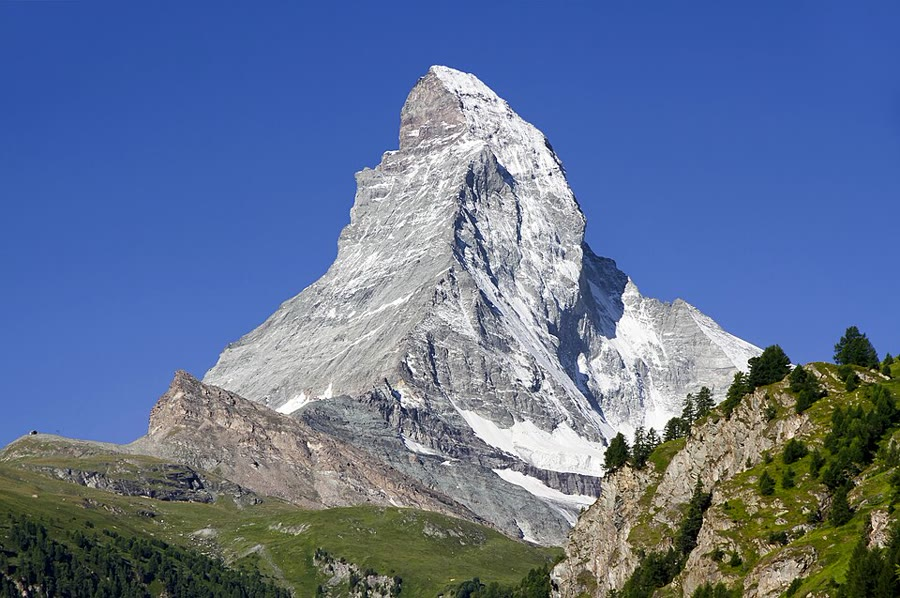
\includegraphics[width=0.7\linewidth]{images/book4/b2-13-matterhorn.jpg}
\par\smallskip{\small A face nordeste do Matterhorn (\qty{4478}{m}), vista de Zermatt:
sua pirâmide superior é gnaisse e gabro apulianos do sistema de cavalgamento da Dent Blanche, uma \omterm{def:b2:alpine-orogen:klippe}{klippe}
sobre os \omterm{def:b2:alpine-orogen:ophiolite}{ofiolitos} do Tétis Alpino. Fotografia de Ximonic (Simo Räsänen), CC BY-SA
4.0.}
\end{omfigure}
% ledger: ispra16:cervino

\subsection*{Descolamentos e as duas peles}

As \omterm{def:b2:alpine-orogen:nappes}{nappes} e as lâminas de cavalgamento se movem sobre superfícies de fraqueza.

\begin{definition}[Descolamento]\label{def:b2:alpine-orogen:decollement}
Um \emph{descolamento}\index{descolamento} (em francês, \textit{décollement}) é uma superfície de baixo ângulo ao longo da qual uma
sequência de rochas se destaca das que estão abaixo e desliza sobre elas, os dois lados se deformando
independentemente; ele geralmente segue uma camada fraca, como um evaporito ou um folhelho.
\end{definition}

\begin{definition}[Tectônica de pele fina e de pele grossa]\label{def:b2:alpine-orogen:skin}
A \emph{tectônica de pele fina}\index{tectônica de pele fina} é a deformação de uma
cobertura sedimentar destacada do seu embasamento ao longo de um \omterm{def:b2:alpine-orogen:decollement}{descolamento} basal: a cobertura se dobra e
cavalga enquanto o embasamento abaixo fica indeformado. A \emph{tectônica de pele
grossa}\index{tectônica de pele grossa} é a deformação na qual o embasamento está envolvido,
cobertura e embasamento se encurtando juntos em falhas que cortam até o embasamento.
\end{definition}
% ledger: lanza22:jura

\begin{definition}[Cinturão de dobras e cavalgamentos]\label{def:b2:alpine-orogen:ftb}
Um \emph{cinturão de dobras e cavalgamentos}\index{cinturão de dobras e cavalgamentos} é um cinturão de dobras e falhas de empurrão
que encurta a parte externa de um \omterm{def:b2:alpine-orogen:orogen}{orógeno} e se propaga em direção ao seu antepaís; os cavalgamentos
sobem em degraus a partir do \omterm{def:b2:alpine-orogen:decollement}{descolamento} através das camadas, e as dobras crescem sobre eles.
\end{definition}

Os Alpes têm as duas peles. As \omterm{def:b2:alpine-orogen:nappes}{nappes} helvéticas são um \omterm{def:b2:alpine-orogen:ftb}{cinturão de dobras e cavalgamentos} de pele fina, os
calcários mesozoicos da margem europeia próxima destacados do seu embasamento. Sua base é
o cavalgamento de Glarus, onde camadas vermelhas permianas repousam sobre \omterm{def:b2:alpine-orogen:foreland}{flysch} cenozoico. No Mioceno, ao
contrário, blocos de embasamento dos maciços externos, embasamento europeu encurtado e espessado (os maciços
do Aar, do Mont Blanc, de Belledonne, do Pelvoux e do Argentera), foram cavalgados para cima com sua
cobertura: cavalgamento de pele grossa.
% ledger: schmid04:units, schmid04:skins, herwegh08:glarus, rosenberg21:massifs

O Jura, o arco de cristas a noroeste do planalto suíço, é o exemplo clássico de pele
fina. No Mioceno Superior e no Plioceno, sua cobertura mesozoica foi dobrada e cavalgada sobre um
\omterm{def:b2:alpine-orogen:decollement}{descolamento} nos evaporitos fracos do Triássico Médio e Superior, enquanto o embasamento abaixo
dele, que continua dos maciços externos sob a bacia da \omterm{def:b2:alpine-orogen:foreland}{Molassa}, não foi envolvido: na
leitura clássica, o empurrão veio dos distantes maciços externos. A sismologia acrescentou desde então
um capítulo de pele grossa. Os terremotos de Saint-Ursanne em 2000 tiveram sua fonte
a menos de um quilômetro de profundidade e um mecanismo de cavalgamento, um cavalgamento raso ativo na cobertura,
enquanto outros estudos encontram falhas do embasamento reativadas desde o fim do Plioceno. Se
o Jura ainda está destacado do seu embasamento é objeto de debate.
% ledger: lanza22:jura, schmid04:skins

\begin{inthefield}[Ler um contato de cavalgamento]
Entre Flims e o Walensee, no leste da Suíça, corre o cavalgamento de Glarus, um dos
mais notáveis grandes cavalgamentos de baixo ângulo dos Alpes. Ao longo dele, camadas vermelhas permianas, o
Verrucano, repousam sobre \omterm{def:b2:alpine-orogen:foreland}{flysch} cenozoico, rochas muito mais antigas sobre rochas mais jovens. Entre elas, uma
faixa fina e fortemente cisalhada de calcário forma o contato: o calcário de Lochseiten, no qual o deslocamento, de pelo menos 30 a
\qty{40}{km}, se concentrou. No século XIX, Heim leu a estrutura como duas enormes
dobras deitadas frente a frente; Escher von der Linth tinha lido um único cavalgamento, e a leitura do cavalgamento prevaleceu. Um geólogo que encontra um contato assim verifica
três coisas: se rochas mais antigas repousam sobre mais jovens, o que nenhum acamamento comum pode fazer;
se as camadas dos dois lados são truncadas no contato; e se o próprio contato
é uma faixa de rocha cisalhada e recristalizada, e não um plano de acamamento.
\end{inthefield}
% ledger: herwegh08:glarus

\section{Bacias de antepaís: flysch e molassa}\label{sec:b2:alpine-orogen:foreland}

Um cinturão de montanhas carrega a placa sobre a qual se apoia, e a placa se curva para baixo à sua frente.

\begin{definition}[Bacia de antepaís; flysch; molassa]\label{def:b2:alpine-orogen:foreland}
Uma \emph{bacia de antepaís}\index{bacia de antepaís} é uma bacia sedimentar alongada que se forma
entre um \omterm{def:b2:alpine-orogen:orogen}{orógeno} e o continente estável à sua frente, onde a placa é curvada para baixo pela
carga do prisma de cavalgamentos; ela é mais profunda junto à frente de cavalgamento e é ela própria
progressivamente cavalgada. O \emph{flysch}\index{flysch} é o preenchimento de águas profundas de uma tal
bacia, sobretudo turbiditos de arenito e folhelho depositados enquanto a bacia está subalimentada.
A \emph{molassa}\index{molassa} é seu preenchimento posterior, marinho raso e continental, sobretudo
conglomerados e arenitos vindos do cinturão em erosão, depositados quando o aporte enche a
bacia.
\end{definition}
% ledger: sinclair97:trinity, schmid04:foreland, krenmayr99:molasse

A curvatura é a flexão elástica da litosfera, tratada num capítulo do terceiro
ano; aqui importa apenas seu efeito sobre a bacia. Sinclair descreveu a primeira \omterm{def:b2:alpine-orogen:foreland}{bacia de antepaís} alpina, de idade paleocena a oligocena,
como uma ``trindade subalimentada'': calcários do lado continental, lama hemipelágica no
meio, turbiditos de águas profundas contra a frente de cavalgamento. À medida que os cavalgamentos avançavam, a bacia
se movia com eles: através da Suíça, sua linha de costa continental avançou para noroeste a 8.5
a \qty{12.9}{mm} por ano, e a bacia migrou com uma forma quase constante por pelo menos
\qty{210}{km} sobre a placa europeia.
% ledger: sinclair97:trinity

A bacia da \omterm{def:b2:alpine-orogen:foreland}{Molassa} do norte dos Alpes, que se estende dos Alpes Marítimos até Viena, começou a
subsidir no Eoceno Superior. O \omterm{def:b2:alpine-orogen:foreland}{flysch} do Oligoceno Inferior, hoje encontrado sobre as \omterm{def:b2:alpine-orogen:nappes}{nappes}
helvéticas, registra uma última fase de águas profundas; do Oligoceno Superior ao Mioceno Superior, rios
espalharam cascalhos e areias continentais vindos das montanhas jovens. O nome é antigo: H.-B. de Saussure
introduziu \emph{molasse} em 1779. O preenchimento se espessa em direção ao cinturão: no
setor austríaco, até mais de \qty{4000}{m} na frente de cavalgamento, e em outros pontos da bacia
uma única sucessão de conglomerados fluviais do Oligoceno Superior tem cerca de \qty{4}{km} de espessura. A parte sul
da bacia foi cavalgada: a faixa aflorante austríaca, com cerca de \qty{60}{km} de largura, é menos
de um quarto da antiga largura da bacia. A própria \omterm{def:b2:alpine-orogen:foreland}{molassa} cavalgada está presa
nos cavalgamentos como a \omterm{def:b2:alpine-orogen:foreland}{Molassa} Subalpina, lascas de conglomerado mergulhando para o sul ao longo da
borda norte do cinturão.
% ledger: schmid04:foreland, krenmayr99:molasse, gs18:conglomerates

Ao sul dos Alpes, a planície do Pó repousa sobre o antepaís adriático, pouco deformado, dos
Alpes Meridionais. Seus sedimentos mais jovens, pliocenos e pleistocenos, cobrem em parte estruturas
alpinas em discordância e são em parte deformados pelos últimos cavalgamentos dos Alpes Meridionais
e dos Apeninos.
% ledger: schmid04:foreland

\begin{omfigure}
\centering
\begin{tikzpicture}[x=0.5cm, y=0.6cm, font=\scriptsize]
\begin{scope}
\node[anchor=west, font=\scriptsize\bfseries] at (0,2.4) {(a) subalimentada: flysch};
\fill[blue!8] (0,0) -- (12,0) -- (12,1.4) -- (9.0,1.4) -- (4,0.05) -- (0,0.05) -- cycle;
\fill[gray!25] (0,0) -- (12,-1.1) -- (12,-1.9) -- (0,-0.8) -- cycle;
\fill[omThm!30] (9.0,1.4) -- (12,2.2) -- (12,-1.1) -- (9.5,-0.87) -- cycle;
\fill[green!25!gray!40] (5.5,-0.5) -- (9.5,-0.87) -- (9.3,-0.35) -- (7.0,-0.2) -- cycle;
\node at (10.9,0.6) {prisma};
\node at (2,-0.45) {cráton};
\node[anchor=north] at (7.3,-0.9) {turbiditos};
\draw[->] (7.3,-0.95) -- (7.6,-0.55);
\end{scope}
\begin{scope}[xshift=6.4cm]
\node[anchor=west, font=\scriptsize\bfseries] at (0,2.4) {(b) sobrealimentada: molassa};
\fill[gray!25] (0,0) -- (12,-1.1) -- (12,-1.9) -- (0,-0.8) -- cycle;
\fill[omThm!30] (8.5,1.6) -- (12,2.4) -- (12,-1.1) -- (9.0,-0.82) -- cycle;
\fill[yellow!40] (1.5,-0.13) -- (9.0,-0.82) -- (8.5,1.0) -- (5,0.35) -- cycle;
\fill[blue!8] (0,0) -- (1.5,-0.13) -- (5,0.35) -- (4,0.4) -- (0,0.4) -- cycle;
\node at (10.6,0.6) {prisma};
\node at (2,-0.45) {cráton};
\node at (6.2,-0.05) {cascalhos, areias};
\end{scope}
\end{tikzpicture}
\par\smallskip{\small Uma \omterm{def:b2:alpine-orogen:foreland}{bacia de antepaís} em duas etapas (esquemático). (a)~No início, a placa
curvada subside mais depressa do que chegam os sedimentos: águas profundas contra o prisma de cavalgamentos, onde
se acumulam turbiditos (\omterm{def:b2:alpine-orogen:foreland}{flysch}). (b)~Mais tarde, o cinturão em erosão fornece mais do que a bacia pode
conter: rios a enchem de cascalhos e areias (\omterm{def:b2:alpine-orogen:foreland}{molassa}), e o prisma cavalga seus próprios
detritos.}
\end{omfigure}
% ledger: sinclair97:trinity, schmid04:foreland

\section{Ler a história: seções e geofísica}\label{sec:b2:alpine-orogen:sections}

Um mapa mostra onde estão as unidades; uma seção geológica mostra como elas se dispõem em profundidade, e ela pode ser
testada.

\begin{definition}[Seção balanceada]\label{def:b2:alpine-orogen:balanced}
Uma \emph{seção balanceada}\index{seção balanceada} é uma seção geológica de rochas
deformadas, traçada paralelamente à direção de transporte, que pode ser restaurada a um estado indeformado geologicamente
razoável sem ganhar nem perder rocha: os comprimentos das camadas-guia e
as áreas das unidades rochosas na seção se conservam entre os estados deformado e
restaurado.
\end{definition}

A restauração é ancorada por \emph{linhas de fixação} (em inglês, \textit{pin lines}), linhas que atravessam as camadas nas extremidades da
seção, escolhidas onde as rochas não deslizaram umas sobre as outras.

\begin{proposition}[Balanço de comprimento e de área]\label{prop:b2:alpine-orogen:balance}
Entre duas linhas de fixação separadas por uma distância $l$ no estado deformado, seja uma camada-guia de
comprimento $l_0$, medido ao longo da camada, e seja uma camada de espessura original $t$ e de área
de seção transversal $A$. Se o comprimento e a área se conservam no plano da seção,
\begin{enumerate}
\item a camada media $l_0$ antes da deformação, o encurtamento é
$e = 1 - l/l_0$ e a distância de encurtamento é $S = l_0 - l$;
\item o comprimento restaurado da camada é $l_0 = A/t$;
\item se um horizonte-guia estava a uma profundidade $d$ acima de um \omterm{def:b2:alpine-orogen:decollement}{descolamento} plano, a área de rocha
erguida acima do nível original do horizonte, sua \emph{área excedente} $A_e$, é igual a $S\,d$;
logo $d = A_e/S$.
\end{enumerate}
\end{proposition}

\begin{omfigure}
\centering
% book's own geometry (figdata/bachelor-2/alps.py)
\begin{tikzpicture}
\begin{axis}[width=0.86\linewidth, height=4.0cm, axis equal image, xmin=-1.5, xmax=31.5,
  ymin=-7.5, ymax=4.8, axis lines=none, clip=false]
\addplot[omThm, line width=1.2pt] table[x=x_km, y=y_km] {figdata/out/bachelor-2-alps-chevron.dat};
\addplot[gray, line width=1.2pt] table[x=x_km, y=y_km] {figdata/out/bachelor-2-alps-chevron0.dat};
\draw[dashed] (axis cs:0,-7) -- (axis cs:0,4.3);
\draw[dashed] (axis cs:22.98,-1.2) -- (axis cs:22.98,4.3);
\draw[dashed] (axis cs:30,-7) -- (axis cs:30,-4.8);
\draw[<->] (axis cs:0,-1.4) -- node[below, font=\scriptsize] {$l = \qty{23.0}{km}$} (axis cs:22.98,-1.4);
\node[font=\scriptsize, anchor=south] at (axis cs:15,-5.9) {restaurada: $l_0 = \qty{30.0}{km}$};
\node[font=\scriptsize, anchor=west] at (axis cs:23.3,2.2) {mergulho dos flancos \qty{40}{\degree}};
\node[font=\scriptsize, anchor=south] at (axis cs:0,4.3) {fixação};
\node[font=\scriptsize, anchor=south] at (axis cs:22.98,4.3) {fixação};
\end{axis}
\end{tikzpicture}
\par\smallskip{\small Balanço de comprimento de uma camada-guia dobrada em chevrons com flancos
mergulhando \qty{40}{\degree} (acima), e a mesma camada restaurada entre suas linhas de fixação
(abaixo), em escala verdadeira. Cada flanco conserva seu comprimento; a camada dobrada se estende por
$l = 30.0\cos\qty{40}{\degree} = \qty{23.0}{km}$, um encurtamento de $1 - \cos\qty{40}{\degree} =
\qty{23.4}{\percent}$.}
\end{omfigure}

\begin{proof}
(1) Uma camada que não se estica nem se encurta ao longo do seu comprimento o conserva; o encurtamento é
a fração de comprimento perdida, como no ensino médio. (2) Antes da deformação, a camada é uma faixa de
comprimento $l_0$ e espessura $t$, de área $l_0 t$, e a área se conserva. (3) Antes da
deformação, a rocha entre o nível do horizonte-guia e o \omterm{def:b2:alpine-orogen:decollement}{descolamento} preenchia uma faixa de $l_0$
de comprimento e $d$ de espessura. Depois dela, entre as linhas de fixação, a mesma rocha preenche uma faixa de $l$ de comprimento,
do \omterm{def:b2:alpine-orogen:decollement}{descolamento} até o nível original do horizonte, de área $l\,d$, mais a área excedente
empurrada acima desse nível. A conservação dá $l_0 d = l\,d + A_e$, logo $A_e = (l_0 -
l)\,d = S\,d$. A relação dá a profundidade de um \omterm{def:b2:alpine-orogen:decollement}{descolamento} oculto a partir de uma área excedente
e de um encurtamento medidos.
\end{proof}


\begin{method}[Restaurar uma seção]\label{met:b2:alpine-orogen:restore}
\begin{enumerate}
\item Escolha-se uma seção paralela à direção de transporte e duas linhas de fixação onde não
houve deslizamento entre as camadas.
\item Meça-se cada camada-guia ao longo do seu comprimento entre as linhas de fixação, contando cada parte
repetida por um cavalgamento.
\item Estendam-se as camadas planas em seus comprimentos medidos, mantendo a ordem das camadas,
e redesenhem-se as falhas na seção restaurada: seus cortes devem se alinhar, sem lacunas
nem sobreposições.
\item Compare-se: camadas de uma mesma lâmina de cavalgamento devem se restaurar no mesmo comprimento; as áreas das
camadas, divididas por suas espessuras, devem dar também os mesmos comprimentos. Uma seção que
falha não é admissível tal como foi traçada.
\end{enumerate}
\end{method}

O balanceamento é um teste de uma seção, não uma prova dela, e suas hipóteses importam. No Jura,
perto do Chasseral, o balanço de comprimento do topo do Jurássico dá \qty{5.1}{km} de
deslocamento, mas o balanço de área e a modelagem direta dão \qty{11.3}{km}: os
\qty{6.2}{km} adicionais foram transportados ao longo de um segundo \omterm{def:b2:alpine-orogen:decollement}{descolamento}, superior, nos folhelhos jurássicos e transmitidos
a dobras mais ao norte. Uma camada-guia tinha deixado escapar metade do movimento. O mesmo estudo
pesou, e não precisou, duas outras leituras comuns no Jura: altos do embasamento empurrando
as dobras para cima, e núcleos de anticlinais espessados por evaporitos triássicos que fluem para dentro deles, um
processo que invalida o balanço de área, pois a camada de evaporitos já não conserva sua
espessura.
% ledger: schori15:chasseral, schori15:evaporite-flow

\subsection*{Quanto encurtamento?}

Aplicado a transectos inteiros, o balanceamento dá o encurtamento total do cinturão, e as respostas
diferem conforme as hipóteses. Através dos Alpes Centrais, ao longo do transecto NFP-20, as estimativas
do encurtamento colisional foram de cerca de \qty{125}{km} em trabalhos anteriores, \qty{160}{km} em
uma compilação de 2015 e \qty{144}{km} em uma revisão de 2021; somar o deslizamento dextral na Linha Periadriática, que
deslocou a Apúlia lateralmente ao longo do cinturão, eleva a convergência total para entre 206 e
\qty{250}{km}, conforme o deslizamento suposto. Nos Alpes Ocidentais, as estimativas
vão de 124 a \qty{243}{km}. Cada uma delas é uma soma de peças restauradas, cada uma com
suas próprias linhas de fixação e suas próprias suposições sobre o que a erosão e a subducção removeram.
% ledger: rosenberg21:shortening

\subsection*{O que a geofísica vê}

As seções em profundidade se apoiam na geofísica. Perfis de sísmica de reflexão profunda foram levantados
através do cinturão (ECORS--CROP nos Alpes Ocidentais, NFP-20 Oeste e Leste na
Suíça, TRANSALP no leste), e redes densas de sismômetros mapeiam hoje o Moho
a partir de funções do receptor, as conversões de ondas P telessísmicas em ondas S na base da
crosta. O mapa AlpArray, construído a partir de mais de cem mil funções do receptor,
encontra o Moho a cerca de \qty{30}{km}, valor típico dos continentes, em torno do cinturão, e a 55 a
\qty{60}{km} sob os Alpes; o Moho europeu mergulha suavemente de cerca de \qty{30}{km} no
noroeste até cerca de \qty{55}{km} sob a cadeia.
A seção esquemática abaixo resume como são lidos os perfis NFP-20 através dos Alpes
Centrais.
% ledger: schmid04:transects, michailos23:moho

\begin{omfigure}
\centering
\begin{tikzpicture}[x=0.6cm, y=0.5cm, font=\scriptsize]
% surface and cover
\fill[yellow!30] (0,0) -- (3.0,0) -- (6.5,-0.3) -- (8.0,0.4) -- (8.0,-0.9) -- (0,-0.6) -- cycle;
\fill[gray!12] (0,-0.6) -- (8.0,-0.9) -- (12.5,-4.5) -- (15,-3.5) -- (16.5,-6.6) -- (16,-8.3)
  -- (0,-5.0) -- cycle;
\fill[gray!35] (0,-5.0) -- (16,-8.3) -- (17.5,-10.0) -- (0,-6.0) -- cycle;
% Helvetic and Aar
\fill[cyan!25] (8.0,0.4) -- (10.0,1.6) -- (11.0,1.2) -- (9.5,-0.4) -- (8.0,-0.9) -- cycle;
\fill[gray!12] (8.0,-0.9) -- (9.5,-0.4) -- (11.0,1.2) -- (12.0,2.0) -- (12.8,0.2) -- (11.5,-1.8)
  -- (12.5,-4.5) -- cycle;
% Penninic stack
\fill[omThm!35] (12.0,2.0) -- (14.5,2.6) -- (17.0,2.2) -- (17.3,-1.0) -- (15.0,-3.5) -- (12.5,-4.5)
  -- (11.5,-1.8) -- (12.8,0.2) -- cycle;
% Austroalpine/Apulia and Southern Alps
\fill[orange!30] (17.0,2.2) -- (19.0,1.6) -- (24,0.2) -- (26,0) -- (26,-3.5) -- (20.5,-4.0)
  -- (17.3,-1.0) -- cycle;
\fill[brown!35] (17.3,-1.0) -- (20.5,-4.0) -- (19.0,-7.0) -- (16.5,-6.6) -- (15,-3.5) -- cycle;
\fill[gray!35] (20.5,-4.0) -- (26,-3.5) -- (26,-6.0) -- (19.0,-7.0) -- cycle;
\fill[yellow!30] (23.5,0.3) -- (26,0) -- (26,-0.5) -- (24.5,-0.3) -- cycle;
\draw[thick] (17.3,-1.0) -- (17.0,2.2);
\draw[thick] (8.0,-0.9) -- (12.5,-4.5);
\draw[dashed] (0,-6.0) -- (17.5,-10.0);
\draw[dashed] (19.0,-7.0) -- (26,-6.0);
\node at (2.2,-0.25) {Jura};
\node at (5.2,-0.35) {molassa};
\node at (9.0,0.15) {Helvético};
\node at (10.6,-0.6) {Aar};
\node at (14.6,0.4) {nappes peninicas};
\node at (21.2,-0.9) {Alpes Meridionais};
\node at (24.9,-0.3) {Pó};
\node at (18.0,-4.8) {Ivrea};
\node[align=center] at (5,-3.0) {crosta europeia};
\node[anchor=north] at (3.2,-7.4) {Moho europeu};
\node at (10,-9.3) {manto};
\node at (23,-7.7) {manto};
\node[anchor=north] at (23,-6.55) {Moho adriático};
\node[anchor=south, align=center] at (17.2,2.25) {Linha\\Periadriática};
\draw[-{Latex[length=2mm]}] (1.0,0.5) -- (0.0,0.5);
\node[anchor=south] at (0.5,0.5) {NO};
\draw[-{Latex[length=2mm]}] (25.0,1.2) -- (26.0,1.2);
\node[anchor=south] at (25.5,1.2) {SE};
\end{tikzpicture}
\par\smallskip{\small Uma seção crustal esquemática através dos Alpes Centrais, do Jura à
planície do Pó (fora de escala; segundo as interpretações dos transectos NFP-20 compiladas por
Schmid e colaboradores). A crosta europeia, com o Jura dobrado e destacado do seu topo, mergulha sob
as \omterm{def:b2:alpine-orogen:nappes}{nappes} helvéticas, o maciço do Aar e a \omterm{def:b2:alpine-orogen:nappes}{pilha de nappes} peninicas; ao sul da Linha
Periadriática, a crosta apuliana com a cunha do corpo de Ivrea fica acima do Moho europeu, e os
Alpes Meridionais cavalgam para o sul sobre a planície do Pó.}
\end{omfigure}
% ledger: schmid04:transects, schmid04:units, schmid04:apulia, schmid04:skins


\begin{omfigure}
\centering
% ledger: data:b4-etopo-alps, data:b4-alps-moho, michailos23:moho
\begin{tikzpicture}
\begin{groupplot}[group style={group size=1 by 2, vertical sep=0.25cm, x descriptions at=edge bottom},
  width=0.92\linewidth, xmin=0, xmax=300, tick label style={font=\scriptsize},
  label style={font=\small}]
\nextgroupplot[height=3.6cm, ymin=0, ymax=4000, ylabel={altitude (\unit{m})},
  ytick={0,1000,2000,3000,4000}, y tick label style={/pgf/number format/1000 sep={}},
  legend style={font=\scriptsize, at={(0.99,0.97)}, anchor=north east, draw=none, fill=none}]
\addplot[gray, line width=0.4pt] table[x=km, y=max_m] {figdata/out/bachelor-2-alps-swath.dat};
\addplot[omThm, line width=1pt] table[x=km, y=mean_m] {figdata/out/bachelor-2-alps-swath.dat};
\legend{máximo da faixa, média da faixa}
\node[font=\scriptsize, anchor=south west] at (axis cs:2,2650) {A (planície do Pó)};
\node[font=\scriptsize, anchor=south east] at (axis cs:298,1500) {B};
\nextgroupplot[height=4.6cm, ymin=0, ymax=70, y dir=reverse, xlabel={distância ao norte de
  \qty{45.3}{\degree} N ao longo de \qty{8}{\degree} L (\unit{km})}, ylabel={profundidade (\unit{km})},
  legend style={font=\scriptsize, at={(0.99,0.03)}, anchor=south east, draw=none, fill=none}]
\addplot[only marks, mark=*, mark size=1.6pt, black] table[x=km, y=moho_km] {figdata/out/bachelor-2-alps-moho.dat};
\addplot[omThm, dashed, line width=0.8pt] table[x=km, y=airy_km] {figdata/out/bachelor-2-alps-airy.dat};
\addplot[gray, densely dotted] coordinates {(0,30) (300,30)};
\legend{Moho observado, previsão de Airy, \qty{30}{km}}
\end{groupplot}
\end{tikzpicture}
\par\smallskip{\small Perfil A--B ao longo de \qty{8}{\degree} L. Acima: altitude média e máxima
dos nós do ETOPO1 numa faixa de \qty{0.25}{\degree} de cada lado do meridiano.
Abaixo: as profundidades do Moho lidas neste meridiano no mapa de funções do receptor do AlpArray
(Michailos e colaboradores, CC BY 4.0), e o Moho que a isostasia local de Airy poria sob
o relevo médio da faixa, para uma crosta de \qty{30}{km} e densidades de 2700 e
\qty{3300}{kg.m^{-3}}.}
\end{omfigure}

O perfil acima confronta a raiz com o modelo de Airy do volume do primeiro
ano. Sob a parte mais alta do perfil, onde o relevo médio da faixa atinge
\qty{2.74}{km} a \qty{46.5}{\degree} N, uma raiz de Airy local poria o Moho a
$30 + 4.5 \times 2.74 = \qty{42.3}{km}$; ele é observado a \qty{36.3}{km}. Cerca de cem
quilômetros mais ao sul, na borda da planície do Pó, onde o relevo médio é de apenas
\qty{0.65}{km}, o Moho observado é o mais profundo do perfil, \qty{61.2}{km}. A raiz não está sob os picos: ela está
deslocada em direção à Apúlia. No trecho onde há leituras, sua seção transversal, medida
abaixo de \qty{30}{km}, é de cerca de \qty{2300}{km^2}, contra cerca de \qty{1500}{km^2} para as raízes de
Airy do relevo acima dela. A compensação local da topografia atual não
explica a raiz. Pfiffner e colaboradores apontam uma carga extra: o corpo de Ivrea, uma cunha de
manto e crosta inferior adriáticos dentro do cinturão, que ajudou a curvar a placa europeia
para baixo.
% ledger: data:b4-etopo-alps, data:b4-alps-moho, michailos23:moho, pfiffner02:ivrea

A gravimetria conta a mesma história de outra maneira. O mapa pan-alpino de anomalia de Bouguer mostra um
mínimo gravimétrico alpino de $-100$ a \qty{-170}{mGal} ao longo da cadeia, mais profundo nos Alpes
Centrais, devido à crosta leve da raiz espessada; um mínimo da bacia do Pó de cerca de $-80$ a
\qty{-140}{mGal}; e, entre os Alpes Ocidentais e a planície do Pó, o estreito máximo gravimétrico de
Ivrea, de até \qty{+40}{mGal}, onde essa crosta inferior e esse manto densos chegam perto da
superfície.
% ledger: zahorec21:gravity

\section{Uma cronologia dos Alpes}\label{sec:b2:alpine-orogen:timeline}

Reunir as datas deste capítulo dá a história do cinturão numa só tabela
(tabela abaixo).

\begin{omfigure}
\centering\small
\begin{tabular}{p{0.28\linewidth}|p{0.62\linewidth}}
época & evento \\ \hline
Jurássico Médio & o oceano Piemonte--Ligúria se abre; seus gabros se cristalizam a
\qty{164}{Ma} \\
início do Cretáceo & o oceano do Valais se abre ao norte do Briançonnais \\
cerca de \qty{100}{Ma} & pico de alta pressão da orogenia cretácea nos Alpes orientais \\
Cretáceo Superior & a margem apuliana (zona Sesia) é subductada; a margem apuliana do
oceano é ativa \\
48 a \qty{44}{Ma} & o fundo oceânico de Zermatt--Saas atinge seu ponto mais profundo, coesita e
diamante em Lago di Cignana \\
Eoceno Médio a Superior & o oceano do Valais se fecha; a bacia da \omterm{def:b2:alpine-orogen:foreland}{Molassa} começa a subsidir \\
\qty{35}{Ma} & crosta continental de Dora Maira em ultra-alta pressão \\
Oligoceno e Mioceno & o cavalgamento de Glarus; cascalhos de \omterm{def:b2:alpine-orogen:foreland}{molassa} enchem o antepaís norte (do Oligoceno
Superior ao Mioceno Superior) \\
Mioceno & soerguimento de pele grossa dos maciços externos; os Alpes Meridionais cavalgam
para o sul \\
Mioceno Superior a Plioceno & dobramento de pele fina do Jura \\
hoje & o nivelamento mostra um soerguimento relativo das rochas de até \qty{1.3}{mm} por ano no núcleo dos
Alpes Centrais
\end{tabular}
\par\smallskip{\small Os Alpes em onze etapas; as fontes são citadas nas seções
acima.}
\end{omfigure}
% ledger: schmid04:alpine-tethys, rubatto98:zsf, schmid04:two-orogenies, halama20:cignana, schmid04:foreland, rh01:exhumation, herwegh08:glarus, schmid04:skins, schmid04:apulia, champagnac09:uplift

A última linha não é o fim da convergência. Nivelamentos repetidos através dos Alpes Centrais
dão um soerguimento relativo das rochas de cerca de \qty{-0.4}{mm} por ano ao norte do Jura a
\qty{1.3}{mm} por ano no núcleo da cadeia, enquanto as medidas de GPS sugerem que os
Alpes Centrais não estão convergindo hoje. Champagnac e colaboradores leem o soerguimento como a recuperação isostática de uma
crosta que está sendo aliviada pela erosão: as montanhas sobem porque são desgastadas.
% ledger: champagnac09:uplift

\section*{Exercícios}\label{sec:b2:alpine-orogen:exercises}

Dados para os exercícios: $g = \qty{9.8}{m.s^{-2}}$,
$G = \qty{6.674e-11}{m^3.kg^{-1}.s^{-2}}$.

\begin{exercise}[$\star$]\label{exo:b2:alpine-orogen:1}
Numa seção geológica, uma camada de calcário medida ao longo de suas dobras entre duas linhas de fixação tem
\qty{36.0}{km} de comprimento; as linhas de fixação estão a \qty{27.0}{km} uma da outra. (a) Usando a
\cref{prop:b2:alpine-orogen:balance}, calcule o encurtamento $e$ e a distância de encurtamento
$S$. (b) O que tem de ser verdade sobre a camada para que a resposta seja válida?
\end{exercise}

\begin{exercise}[$\star$]\label{exo:b2:alpine-orogen:2}
Num mapa geológico, (a) uma mancha oval de gnaisse de \qty{4}{km} de comprimento repousa sobre calcário
jurássico, com um contato que é um cavalgamento mergulhando para dentro, sob o gnaisse, em todo o contorno; (b) uma
área alongada de folhelho cretáceo é cercada por gnaisse, ao longo de um cavalgamento que mergulha
para fora, sob o gnaisse, em todo o contorno. Nomeie cada estrutura e diga o que a erosão fez
em cada caso.
\end{exercise}

\begin{exercise}[$\star$]\label{exo:b2:alpine-orogen:3}
(a) Liste as quatro unidades da \omterm{def:b2:alpine-orogen:ophiolite}{sequência ofiolítica de Penrose} da base para o topo, e associe cada uma
a uma camada da crosta oceânica ou do manto. (b) O \omterm{def:b2:alpine-orogen:ophiolite}{ofiolito} do Chenaillet mostra manto
exposto, gabro e basaltos em almofada, e nenhuma cobertura sedimentar. Que unidade de Penrose essa
lista deixa de fora? (c) Por que os \omterm{def:b2:alpine-orogen:ophiolite}{ofiolitos} não dão uma amostra representativa do fundo dos
oceanos largos?
\end{exercise}
% ledger: coleman84:penrose, coleman84:settings, corno23:chenaillet

\begin{exercise}[$\star$]\label{exo:b2:alpine-orogen:4}
Subindo o Matterhorn pelo sul, um alpinista atravessa sucessivamente as \omterm{def:b2:alpine-orogen:nappes}{nappes} do Monte Rosa e do
Grand St Bernard, os \omterm{def:b2:alpine-orogen:ophiolite}{ofiolitos} de Zermatt--Saas, a zona do Combin e os gnaisses do sistema de
cavalgamento da Dent Blanche. (a) Dê o domínio de origem de cada um. (b) Que placa era
a placa superior durante a subducção? (c) Por que essa ordem é uma regra geral na \omterm{def:b2:alpine-orogen:nappes}{pilha de nappes},
e o que pode quebrá-la?
\end{exercise}
% ledger: ispra16:cervino, schmid04:units

\begin{exercise}[$\star\star$]\label{exo:b2:alpine-orogen:5}
Os Alpes Centrais apresentam uma anomalia de Bouguer de cerca de \qty{-170}{mGal}. (a) Usando a placa
de Bouguer do volume do primeiro ano, $\Delta g = 2\pi G\,\Delta\rho\,h$, encontre a espessura $h$ de uma
placa infinita com déficit de densidade $\Delta\rho = \qty{500}{kg.m^{-3}}$ (crosta substituindo manto)
que dá essa anomalia. (b) As funções do receptor mostram uma raiz de cerca de \qty{25}{km} abaixo de uma
crosta de \qty{30}{km}. Que anomalia daria uma placa infinita dessa espessura? (c) Por que a
anomalia observada é menor?
\end{exercise}
% ledger: zahorec21:gravity, michailos23:moho

\begin{exercise}[$\star\star$]\label{exo:b2:alpine-orogen:6}
Gabros do \omterm{def:b2:alpine-orogen:ophiolite}{ofiolito} de Zermatt--Saas se cristalizaram a \qty{164}{Ma}; o \omterm{def:b2:alpine-orogen:ophiolite}{ofiolito} atingiu
seu ponto mais profundo a \qty{44}{Ma}, a \qty{2.8}{GPa}. (a) Que idade tinha a litosfera
oceânica quando foi subductada? (b) Converta a pressão em profundidade com uma densidade média de
sobrecarga de \qty{3000}{kg.m^{-3}}, depois de \qty{3300}{kg.m^{-3}}. (c) Compare com os
``mais de \qty{90}{km}'' citados para essa rocha.
\end{exercise}
% ledger: rubatto98:zsf, halama20:cignana

\begin{exercise}[$\star\star$]\label{exo:b2:alpine-orogen:7}
Uma camada está dobrada em chevrons cujos flancos retos mergulham todos com o ângulo $\theta$.
(a) Mostre que o encurtamento é $e = 1 - \cos\theta$. (b) Que mergulho dos flancos dá
\qty{30}{\percent} de encurtamento? (c) Que encurtamento dão flancos mergulhando \qty{40}{\degree} e
\qty{60}{\degree}? Confira o primeiro com a figura dos chevrons da seção sobre o balanceamento.
\end{exercise}

\begin{exercise}[$\star\star$]\label{exo:b2:alpine-orogen:8}
Uma cobertura de \qty{2.0}{km} de espessura está dobrada e cavalgada sobre um \omterm{def:b2:alpine-orogen:decollement}{descolamento} plano. Entre linhas de fixação
hoje a \qty{42}{km} uma da outra, sua área em seção é de \qty{118}{km^2}. (a) Encontre seu comprimento
restaurado, $S$ e $e$. (b) Calcule a área excedente e a profundidade do \omterm{def:b2:alpine-orogen:decollement}{descolamento} abaixo do
topo original da cobertura. (c) O resultado é coerente?
\end{exercise}

\begin{exercise}[$\star\star$]\label{exo:b2:alpine-orogen:9}
Ao longo do perfil a \qty{8}{\degree} L deste capítulo, a altitude média da faixa é de
\qty{2.74}{km} a \qty{46.5}{\degree} N, onde o Moho é lido a \qty{36.3}{km}, e de
\qty{0.65}{km} a \qty{45.55}{\degree} N, onde ele é lido a \qty{61.2}{km}. (a) Com uma
crosta de referência de \qty{30}{km}, $\rho_c = \qty{2700}{kg.m^{-3}}$ e $\rho_m =
\qty{3300}{kg.m^{-3}}$, calcule a profundidade do Moho de Airy nos dois lugares. (b) Compare com as
leituras. (c) O que a comparação diz sobre como a raiz alpina é sustentada?
\end{exercise}
% ledger: data:b4-etopo-alps, data:b4-alps-moho, pfiffner02:ivrea

\begin{exercise}[$\star\star\star$]\label{exo:b2:alpine-orogen:10}
Na seção do Chasseral, no Jura, o balanço de comprimento do topo do Jurássico
dá \qty{5.1}{km} de deslocamento; o balanço de área e a modelagem dão \qty{11.3}{km}, dos
quais \qty{6.2}{km} foram transportados ao longo de um \omterm{def:b2:alpine-orogen:decollement}{descolamento} superior nos folhelhos do Jurássico Médio.
(a) Que fração do deslocamento a camada do topo do Jurássico registrou? (b) Mostre que os
números fecham, e explique por que a camada superior deixa escapar parte do movimento. (c) Que
lição geral isso dá para o balanceamento com uma única camada-guia?
\end{exercise}
% ledger: schori15:chasseral

\begin{exercise}[$\star\star\star$]\label{exo:b2:alpine-orogen:11}
Através dos Alpes Centrais, foram estimados cerca de \qty{200}{km} de encurtamento dirigido para o norte,
e a Linha Periadriática tem um rejeito dextral leste--oeste de cerca de
\qty{100}{km}, talvez 50, talvez 150. (a) Some os dois como vetores perpendiculares e dê
a convergência total para cada rejeito. (b) Que ângulo a convergência faz com a
direção norte--sul para um rejeito de \qty{100}{km}? (c) Por que a escolha do rejeito
importa mais do que o terceiro algarismo significativo do encurtamento?
\end{exercise}
% ledger: rosenberg21:shortening

\begin{exercise}[$\star\star\star$]\label{exo:b2:alpine-orogen:12}
A parte suíça da \omterm{def:b2:alpine-orogen:foreland}{bacia de antepaís} alpina migrou pelo menos \qty{210}{km} para noroeste
sobre a Europa, com sua linha de costa avançando a 8.5 a \qty{12.9}{mm} por ano. (a) Por que intervalo de
durações durou a migração? (b) No setor austríaco, a faixa aflorante atual,
com cerca de \qty{60}{km} de largura, é menos de um quarto da antiga largura da bacia. Qual era a
menor largura antiga possível, e quanto da bacia está escondido sob os cavalgamentos? (c) Por que uma
\omterm{def:b2:alpine-orogen:foreland}{bacia de antepaís} nunca pode ser preservada por inteiro?
\end{exercise}
% ledger: sinclair97:trinity, krenmayr99:molasse

\begin{problem}[{Problema de fim de semana --- restaurar a seção}]\label{pb:b2:alpine-orogen:1}
Um \omterm{def:b2:alpine-orogen:orogen}{orógeno} de tipo alpino é atravessado por uma seção-modelo (uma geometria inventada pelo próprio livro,
indicada como modelo) composta de cinco domínios, do antepaís ao lado oposto:
um \omterm{def:b2:alpine-orogen:ftb}{cinturão de dobras e cavalgamentos} de antepaís, hoje com \qty{48}{km} de largura; uma \omterm{def:b2:alpine-orogen:nappes}{pilha de nappes} externas, \qty{15}{km};
um maciço de embasamento, \qty{22}{km}; uma zona interna de \omterm{def:b2:alpine-orogen:nappes}{nappes} continentais e \omterm{def:b2:alpine-orogen:ophiolite}{ofiolitos},
\qty{20}{km}; e uma retrocunha com vergência para o sul, \qty{48}{km}
(figura abaixo). Os comprimentos estão em quilômetros do início ao fim.

\begin{omfigure}
\centering
\begin{tikzpicture}[x=0.075cm, y=0.5cm, font=\scriptsize]
\fill[yellow!30] (0,0) rectangle (48,1);
\fill[cyan!25] (48,0) rectangle (63,1);
\fill[gray!25] (63,0) rectangle (85,1);
\fill[omThm!35] (85,0) rectangle (105,1);
\fill[orange!30] (105,0) rectangle (153,1);
\draw (0,0) rectangle (153,1);
\foreach \x in {48,63,85,105} \draw (\x,0) -- (\x,1);
\node at (24,0.5) {cinturão de antepaís};
\node[align=center] at (55.5,1.6) {nappes};
\node at (74,0.5) {maciço};
\node[align=center] at (95,1.6) {zona interna};
\node at (129,0.5) {retrocunha};
\node[anchor=north] at (24,0) {48}; \node[anchor=north] at (55.5,0) {15};
\node[anchor=north] at (74,0) {22}; \node[anchor=north] at (95,0) {20};
\node[anchor=north] at (129,0) {48};
\end{tikzpicture}
\par\smallskip{\small A seção-modelo do problema de fim de semana: larguras atuais dos seus
cinco domínios, em quilômetros (153 ao todo; uma geometria inventada).}
\end{omfigure}

\noindent\textbf{Parte I --- Balanço de comprimento do cinturão de antepaís.} Entre suas duas linhas
de fixação, a \qty{48.0}{km} uma da outra, o topo do calcário principal é formado por dez segmentos retos
(extensão horizontal $\Delta x$, mergulho), listados a partir do antepaís; além disso, uma lâmina de cavalgamento
cobre um trecho plano da mesma camada, de \qty{6.0}{km} de comprimento, que se repete por baixo dela.

\smallskip
\begin{center}\small
\begin{tabular}{l|cccccccccc}
segmento & 1 & 2 & 3 & 4 & 5 & 6 & 7 & 8 & 9 & 10\\ \hline
$\Delta x$ (\unit{km}) & 8.0 & 3.0 & 3.0 & 5.0 & 2.5 & 2.5 & 6.0 & 4.0 & 4.0 & 10.0\\
mergulho (\unit{\degree}) & 0 & 35 & 35 & 0 & 50 & 50 & 10 & 40 & 40 & 5
\end{tabular}
\end{center}
\smallskip

\begin{enumerate}
\item Calcule o comprimento ao longo da camada dos segmentos 2, 5 e 8.
\item Calcule o comprimento total da camada entre as linhas de fixação, incluindo o trecho
repetido.
\item Por que o trecho escondido sob a lâmina de cavalgamento deve ser contado?
\item Calcule o encurtamento $e$ e a distância de encurtamento $S$ do cinturão de antepaís.
\item A base do calcário, medida da mesma maneira, tem \qty{60.2}{km} de comprimento. De quanto,
e de que porcentagem, as duas camadas discordam? A seção é aceitável?
\item O que teria significado um comprimento de \qty{54.0}{km} para a base?
\end{enumerate}

\noindent\textbf{Parte II --- Balanço de área e o descolamento.} A cobertura entre o
\omterm{def:b2:alpine-orogen:decollement}{descolamento} e o topo do calcário tinha \qty{2.4}{km} de espessura antes da deformação; sua
área entre as linhas de fixação é medida como \qty{146}{km^2}.
\begin{enumerate}[resume]
\item Calcule o comprimento restaurado da cobertura a partir da sua área.
\item Compare com o resultado do balanço de comprimento da questão~2.
\item Calcule a área excedente, erguida acima do topo original da cobertura.
\item Deduza a profundidade do \omterm{def:b2:alpine-orogen:decollement}{descolamento} abaixo desse nível, e compare-a com a espessura
da cobertura.
\item Se a área fosse de \qty{160}{km^2}, que comprimento restaurado ela daria? Que processo,
citado no Jura, poderia fazer a área e o comprimento discordarem dessa maneira?
\item Por que este cinturão é de pele fina, e como deveria ser o topo do embasamento
abaixo dele?
\end{enumerate}

\noindent\textbf{Parte III --- As nappes externas e seu ritmo.} A camada-guia das
três \omterm{def:b2:alpine-orogen:nappes}{nappes} externas se restaura em 22, 18 e \qty{25}{km}; a pilha abrange hoje
\qty{15}{km}. No maciço de embasamento, o topo do embasamento se restaura em \qty{30}{km}
contra \qty{22}{km} hoje. O cinturão de antepaís se deformou entre 11 e \qty{4}{Ma}, as
\omterm{def:b2:alpine-orogen:nappes}{nappes} entre 30 e \qty{20}{Ma}.
\begin{enumerate}[resume]
\item Calcule o comprimento restaurado da \omterm{def:b2:alpine-orogen:nappes}{pilha de nappes} e sua distância de encurtamento.
\item Calcule seu encurtamento $e$ e compare-o com o do cinturão de antepaís.
\item Calcule o encurtamento do maciço de embasamento. Que tipo de tectônica é esse?
\item Calcule as taxas médias de encurtamento do cinturão de antepaís e das \omterm{def:b2:alpine-orogen:nappes}{nappes}, em
milímetros por ano.
\item Em que direção a deformação migrou através da seção? Essa é a ordem
dos Alpes?
\item Some os encurtamentos dos três domínios externos.
\end{enumerate}

\noindent\textbf{Parte IV --- A zona interna, o oceano e a seção inteira.}
Lascas de \omterm{def:b2:alpine-orogen:ophiolite}{ofiolito} na zona interna se restauram em \qty{18}{km}. Suponha que o oceano tenha sido
subductado de 85 a \qty{45}{Ma} a uma taxa média de \qty{0.5}{cm} por ano. As \omterm{def:b2:alpine-orogen:nappes}{nappes}
continentais da zona interna se restauram em \qty{60}{km} contra \qty{20}{km} hoje, e a
camada-guia da retrocunha em \qty{70}{km} contra \qty{48}{km}.
\begin{enumerate}[resume]
\item Que comprimento de litosfera oceânica foi subductado?
\item Dê uma largura mínima para o oceano.
\item Por que é apenas um mínimo?
\item Calcule o encurtamento da zona interna e o da retrocunha.
\item Some o encurtamento colisional dos cinco domínios, e compare-o com as
estimativas para os Alpes Centrais deste capítulo.
\item Verificação crustal: restaure a seção em toda a sua largura com uma crosta de \qty{30}{km}, e
compare a área crustal com a de hoje, uma média de \qty{45}{km} sobre os
\qty{153}{km} atuais. Que fração da crosta falta na seção atual, e para onde
ela foi? Dê o encurtamento colisional total através da seção, arredondado ao
quilômetro.
\end{enumerate}
\end{problem}
